\chapter{Introduzione}

\section{Reti Sottomarine}
Introduciamo il concetto di UWSNs, ovvero Underwater Wireless  Sensor Networks, con il quale intendiamo definire una rete di sensori e veicoli, di diversa natura ed in numero variabile, disposti in una limitata area sottomarina e capaci, in maniera collaborativa, di realizzare una certa missione che imponga la necessita' di comunicare fra i diversi componenti della rete.\newline
I diversi nodi della rete, la cui natura puo' variare da sensori fissati al fondale marino a veri e propri veicoli sottomarini autonomi (Autonomous Underwater Vehicle, AUV), debbono possedere la capacita' di adattarsi in maniera autonoma alle caratteristiche cangianti dell'ambiente in cui vengono utilizzati, scambiando fra loro ed elaborando informazioni riguardo posizionamento, movimento dei nodi mobili e configurazione propria di ciascuno di essi, al fine di coordinare efficacentemente il proprio lavoro e, se necessario, comunicare dati utili alle postazioni sulla terraferma.

\subsection{Applicazioni delle UWSNs}
Le reti sottomarine trovano applicazione in vari contesti, dalla raccolta di dati scientifici al monitoraggio e sorveglianza di una data area sottomarina, fino all'utilizzo nell'ambito dell'archeologia subacquea \cite{underwater}.\newline
Riportiamo un breve elenco delle situazioni d'utilizzo comuni per questo tipo di tecnologia:\newline
\begin{itemize}
\item Monitoraggio Ambientale:  \newline
Raccolta di dati riguardo le caratteristiche fisiche, chimiche e biologiche di un area marina, al fine di valutarne il livello d'inquinamento e l'effetto dell'attivita' umana sull'ecosistema marino\newline
\item Esplorazione del fondale marino: \newline
Esplorazione subacquea al fine di ricerca di riserve di combustibili fossili e posizionamento cavi sottomarini per telecomunicazioni\newline
\item Prevenzione di disastri:\newline
Monitoraggio di area ad alto rischio sismico/vulcanico, in modo da poter studiare piu' efficacemente questi fenomeni naturali e poter disporre di un meccanismo d'allarme per le zone costiere in caso di tsunami\newline
\item Assitenza alla navigazione: \newline
Identificazione degli elementi di pericolo alla navigazione (scogli, fondali bassi, relitti affondati)\newline
\item Sorveglianza:\newline
Reti di nodi fissi e AUVs possono effettuare il monitoraggio di un'area assegnata provvedendo a compiti di sorveglianza, riconoscimento di oggetti all'interno dell'area, individuazione di obbiettivi sensibili e rilevamento di intrusi all'interno dell'area
\end{itemize}
Rispetto alle tecnologie preesistenti in questi campi d'azione (sistemi radar/sonar), queste reti di sensori sottomarini possono ricorrere ad un piu' ampio spettro qualitativo di dati (provenienti da sensori acustici, di radiazioni, di campi magnetici, sensori meccanici), raggiungendo un piu' alto grado di accuratezza nella rilevazione e classificazione di oggetti all'interno dell'area di sorveglianza.\newline

\subsection{Caratteristiche peculiari delle UWNSs e principali difficolta' progettuali}
Gli approcci tradizionali per la progettazione di sistemi che realizzano le funzioni sopra elencate sono accumunati da un approccio architetturale basato sul dispiegamento di sensori fissi, la raccolta di dati per un certo lasso di tempo, il recupero dei sensori e la successiva analisi dei dati accumulati.\newline
Le UWNSs ovviano ad alcuni limiti di questa tipologia di sistemi, nello specifico: \newline
\begin{itemize}
\item Introducono la possibilita' di effettuare monitoraggio ed analisi dei dati in real-time, tramite la comunicazione dei dati a terra (caratteristica innovativa nei sistemi di monitoraggio di zone sismiche, ad esempio)\newline
\item L'interazione costante o cadenzata del personale scientifico con la rete di sensori ne permette la verifica per quanto riguarda il corretto funzionamento della strumentazione. \newline In questo modo si possono effettuare riconfigurazioni dei sistemi on-the-fly ed individuare eventuali malfunzionamenti dei sensori non appena questi si verificano (non dovendo piu' attendere il recupero dei sensori stessi)\newline
\item Viene meno la necessita' di capacita' di storage locali importanti per i sensori, avendo questi la possibilita' di trasmettere i dati accumulati e quindi cancellarli per far posto ad altri rilevamenti
\end{itemize}
Le comunicazioni in questo tipo di reti avvengono solitamente tramite canale acustico. La scelta' di questo tipo di trasmissione e' praticamente obbligata dai limiti presenti nelle trasmissioni di tipo ottico ed elettromagnetico. Le prime soffrono di problemi legati a fenomeni di diffusione ottica.  Invece le onde elettromagnetiche, nel mezzo sottomarino, presentano un forte effetto di attenuazione, proporzionale alla distanza di trasmissione. La propagazione di onde elettromagnetiche in acqua per lunghe distanze potrebbe avvenire percio' solamente a frequenze molto basse (30-300 Hz), il che richiederebbe antenne ingombranti e un elevato dispendio energetico.

La trasmissione tramite onde acustiche si presenta quindi come l'unica soluzione tecnicamente avallabile nelle reti di comunicazione sottomarine. La peculiarita' del mezzo, altresi', impone comunque particolare attenzione nella progettazione di protocolli di rete affidabili, a causa di alcune importanti limitazioni:
\begin{itemize}

\item La banda di trasmissione disponibile fortemente limitata

\item Fenomeni di trasmissione multi-path

\item Tasso di errore nella trasmissione elevato e frequente presenza di zone d'ombra

\item Disponibilita' energetica limitata

\item Ritardo di propagazione altamente variabile e di cinque ordini di grandezza piu' elevato rispetto alle comunicazioni radio terrestri
\end{itemize}

Non ultimo va ricordato che il canale di comunicazione acustico e' ovviamente da intendersi come canale ad accesso condiviso e, come anche le comunicazioni wireless elettromagnetiche, necessita di protocolli che gestiscano l'accesso concorrente al mezzo da parte di piu' nodi. Soluzioni che riprendono l'uso di pacchetti di tipo RTS e CTS, similarmente a quanto specificato dallo standard IEEE 802.11, non sono facilmente implementabili in ambiente underwater sia a causa dell'elevato delay che introdurrebbero (data la bassa capacita' di una rete acoustica sottomarina) sia perche' sono molto piu' frequenti, rispetto alle normali reti wireless, fenomeni di "shadowing" temporaneo dei nodi della rete. Le ricerche recenti propendono invece per l'utilizzo di meccanismi di tipo TDMA e Slotted Aloha che, al costo di una bassa efficienza nell'utilizzo del canale e di una maggiore complessita' d'implementazione, garantiscono l'accesso condiviso al canale senza la necessita' di invio di pacchetti di controllo.

\subsection{Caratteristiche del canale acustico}
Vale la pena dedicare un paragrafo a parte per la descrizione delle caratteristiche peculiari del canale trasmissivo acustico. Le trasmissioni acustiche sono principalmente influenzati da fenomeni di attenuamento, rumore, percorsi multipli, ritardi di propagazione elevati e variabili, problemi dovuti all'effetto Doppler.\newline
Tutto questo rende il canale altamente variabile rispetto al tempo ed allo spazio. I collegamenti che utilizzano il canale acustico sono classificati  in base alla distanza della trasmissione e in base alla direzione, verticale od orizzontale. Ulteriore parametro caratterizzante e' la profondita' della trasmissione (sotto o sopra i 100m di profondita').\newline
Per quanto riguarda l'attenuazione, essa dipende in primis dalla conversione dell'energia acustica in calore. L'attenuazione aumenta con l'aumentare della frequenza di trasmissione e la distanza. 
L'altro fattore principale che causa che l'attenuazione del segnale e' l'espansione del fronte d'onda della comunicazione, che assume una geometria sferica in acque profonde ed una cilindrica in acque poco profonde.\newline
L'elevata presenza di rumore, come anticipato, caratterizza il canale acustico. In parte questo e' causato dalla presenza antropogenica (navi, barche da pesca, impianti sottomarini) ma in maggior parte deriva dall'attivita' idrodinamica marina (correnti, maree, tempeste, onde) ed a quella biologica e sismica.\newline
Col fenomeno dei percorsi multipli si intende l'arrivo di uno stesso segnale al ricevitore in due momenti diversi, a causa di diversi percorsi seguiti dall'onda nella sua propagazione (ad esempio per effetto  di riflessioni). Cio' causa interferenza nella ricezione del segnale e quindi una degradazione della qualita' dello stesso.\newline
In ultimo, il verificarsi di effetti Doppler con diverse traslazioni di frequenza rende difficoltoso per un ricevitore ricostruire il segnale ricevuto (fenomeno che non si verificherebbe in presenza di un effetto Doppler con una singola traslazione di frequenze).

\subsubsection{Caratterizzazione dell'attenuazione e del rumore del canale acustico}
\par
Per completezza, diamo qui una breve caratterizzazione dei fenomeni d'attenuazione che influenzano la comunicazione attraverso il mezzo acustico. A differenza di altre forme di comunicazione wireless, l'attenuazione della potenza di un'onda acustica dipende fortemente non solo dalla distanza fra l'emettitore del segnale ed il ricevitore, ma anche dalla frequenza del segnale: questa determina la quantita' di energia acustica (meccanica) che si trasforma in calore. L'energia assorbita dal mezzo aumenta con l'aumentare della frequenza di trasmissione del segnale (oltre che con l'aumentare della distanza), limitando come vedremo la banda disponibile per la trasmissione.

L'attenuazione per un segnale acustico in ambiente sottomarino trasmesso ad una distanza $l$ e frequenza $f$ e' modellata dalla seguente formula:
\[A(l, f) = A_0 l^k a(f)^l\]
dove $k$ e' il fattore di diffusione del fronte dell'onda acustica (dipende dalla geometria del fronte), $A_0$ e' una costante di normalizzazione e $a(f)$ e' il fattore d'assorbimento specifico per la frequenza.
Esprimendo il valore in decibel otteniamo:
\[10log\ A(l, f)/A_0 = k \cdot 10log\ l + l \cdot 10log\ a(f)\]
Il primo termine rappresenta la dispersione d'energia dovuta alla diffusione dell'onda (k e' uguale ad 1 per fronte d'onda cilindrico, 2 per fronte sferico. 1.5 e' il valore che viene utilizzato nella pratica). Il secondo termine invece dipende dalla frequenza del segnale e, come anticipato, pesa maggiormente sull'attenuazione man mano che la frequenza aumenta.

\begin{figure}[H]
    \centering
    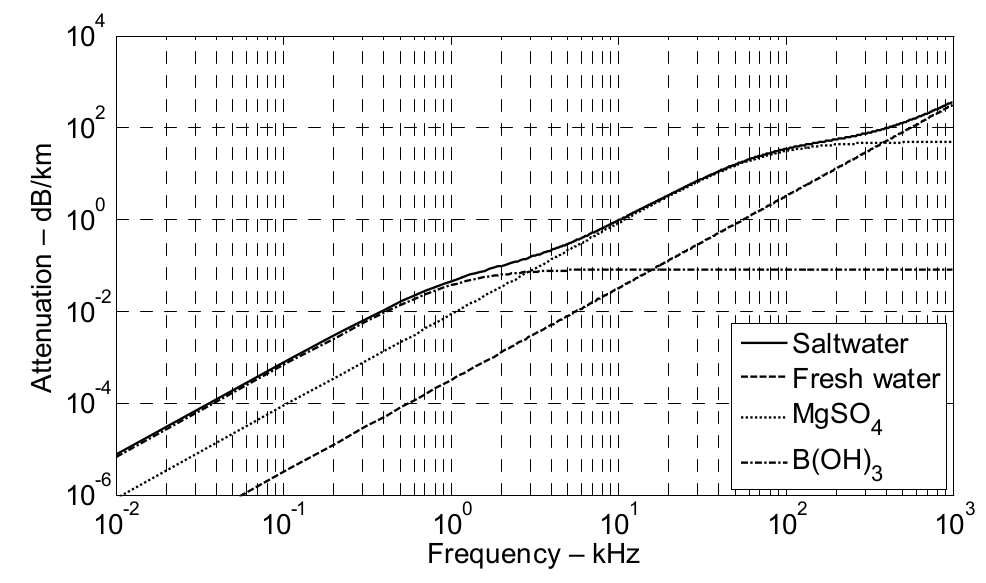
\includegraphics[scale=1.4]{waterabsorption.jpeg}
    \caption{Coefficiente d'assorbimento specifico per la frequenza in varie tipologia d'acqua}
\end{figure}

Un segnale trasmesso con potenza $P$ verra' ricevuto, attenuato, con potenza $P/A(l, f)$.
\par
Per quanto riguarda il rumore da cui un segnale in acqua viene affetto, possiamo considerarlo proveniente da quattro diverse sorgenti principali:
\begin{itemize}
    \item Turbolenza in acqua: $10log\ N_t(f) = 17 - 30log\ f$
    \item Navi di passaggio: $10log\ N_s(f) = 40 + 20(s - 0.5) + 26log\ f - 60log\ (f+0.03)$
    \item Onde: $50 + 7.5w^{1/2}+ 20logf - 40log\ (f+0.4)$
    \item Rumore termico: $-15 + 20logf$
\end{itemize}
Come vediamo, le intensita' delle diverse sorgenti di rumore dipendono, ciascuna in maniera diversa, dalla frequenza del rumore e inficiano dunque su spettri di frequenze differenti. La turbolenza del movimento dell'acqua ha effetto a frequenze molto basse, mentre il rumore generato dal passaggio di navi e' da considerarsi non trascurabile fra i 10 ed i 100 $Hz$ (dipende anche da un fattore di "attivita' navale" $s$, compreso fra 0 ed 1). Il rumore generato dalle onde e' predominante nel range di frequenze tra i 100 $Hz$ e i 100 $kHz$, mentre quello termico lo diviene oltre i 100 $kHz$.
\begin{figure}[H]
    \centering
    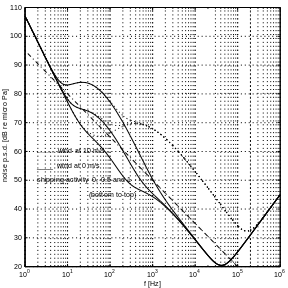
\includegraphics[]{noise.png}
    \caption{Densita' di potenza del rumore totale rispetto alla frequenza}
\end{figure}
Come si nota chiaramente dal grafico, il rumore diminuisce con l'aumentare della frequenza, fornendo cosi' una sorta di limite inferiore alla banda di frequenze da utilizzare per la trasmissione.
\par
Avendo ora descritto sia l'attenuazione del segnale sia il rumore che incide su di esso, possiamo in ultimo valutare il rapporto segnale/rumore di un segnale acustico in acqua (Signal-to-noise-ratio, SNR).
Sia $P$ la potenza di trasmissione del segnale, avremo:
\[SNR(l, f) = \frac{P/A(l, f)}{N(f)\Delta f}\]
dove $\Delta f $ e' una piccola banda di frequenze intorno ad $f$. Il fattore $1/A(l, f)N(f)$ ci indica l'andamento del SNR. Fissando la distanza di trasmissione $l$, per ciascuno di questi valori otteniamo uno specifico andamente dell'SNR in base alla frequenza $f$. Come vediamo, per ciascuna distanza esiste una specifica frequenza $f_0(l)$ per la quale il valore di $1/A(l, f)N(f)$ (e quindi dell'SNR) e' massimo.
\begin{figure}[H]
\centering
    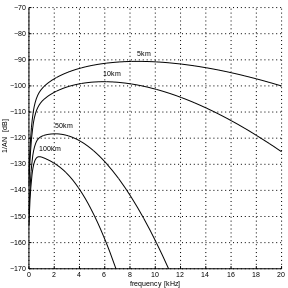
\includegraphics[]{snr.png}
    \caption{Andamento di 1/AN (SNR) rispetto alla frequenza per varie distanza considerate}
\end{figure}

La frequenza ottimale $f_0$ diminuisce con l'aumentare della distanza della trasmissione.
\begin{figure}[H]
    \centering
    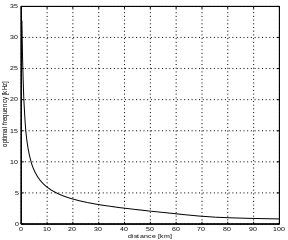
\includegraphics[]{optimalfreq.png}
    \caption{Frequenza ottimale di funzionamento rispetto alla distanza della comunicazione}
\end{figure}
\par
Nell'ambiente simulativo di cui ci si e' serviti per testare il protocollo sviluppato, il canale di comunicazione acustico e le caratteristiche appena descritte vengono rese rifacendosi al modello di Urick \cite{urick}, che fornisce una serie di formule empiriche per modellare al meglio il canale di trasmissione.

\subsection{Modelli di architetture di UWSNs}
In questo paragrafo vengono brevemente presentate tre possibili architetture per le reti di sensori sottomarini \cite{underwater}. L'architettura e la topologia di rete risultano fondamentali nel determinare fattori quali il consumo energetico complessivo della rete, la sua capacita' di trasporto e la sua affidabilita'. \newline Come anticipato, vengono qui prese in esame tre tipi di rete, che si differenziano sia per quanto riguarda la tipologia di nodi impiegati sia la loro diposizione nello spazio.  La prima di queste e' una tipologia di rete con una topologia bidimensionale composta solamente da nodi fissi ancorati al fondale marino.

\begin{figure}[H]
    \centering
	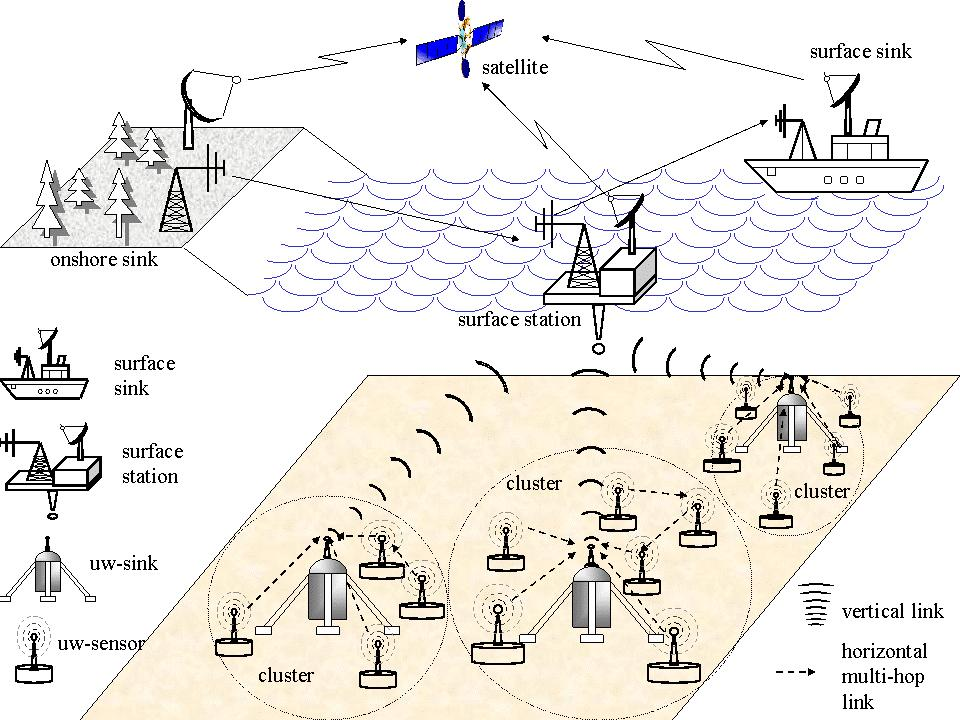
\includegraphics[scale=0.3]{2D_arch.jpg}
	\caption{ Topologia nodi fissi 2D}
	\label{fig:}
\end{figure}

Questi sensori, dotati di modem acustici, sono connessi a degli underwater sinks (uw-sinks nella figura). Questi ultimi svolgono la funzione di ``collettori'' dei dati trasmessi dai sensori, instradandoli verso la superficie marina dove vengono raccolti da una stazione ivi posta. Da notare come gli uw-sinks debbano essere dotati di due modem acustici, uno per le trasmissioni orizzontali con i sensori posizionati sul fondale ed uno per le trasmissioni verticali con la stazione di superficie (quest'ultimo e' spesso un modem per trasmissioni a lungo raggio, vista la profondita operazionale dell'uw-sink). La stazione di superficie comunica contemporaneamente con diversi uw-sink e puo' trasmettere i dati ricevuti direttamente a terra, ad una nave d'appoggio o ad un satellite.
In questo tipo di reti, spesso capita che un sensore non si trovi in prossimita' di un uw-sink ergo la comunicazione diretta con quest'ultimo sarebbe pesantemente inficiata dall'attenuazione dovuta all'elevato range di trasmissione. Una soluzione solitamente adottata in questi casi consiste nel far svolgere ai sensori anche la funzione di routing, consentendo percorsi multi-hop da un sensore verso l'uw-sink di riferimento (cio' ovviamente aumenta la complessita' del protocollo di trasmissione dei dati e dell'elaborazione di ciascun sensore).

La seconda tipologia di rete analizzata consiste ancora di soli sensori fissi, ma questa volta organizzati in uno spazio tridimensionale.

\begin{figure}[H]
    \centering
	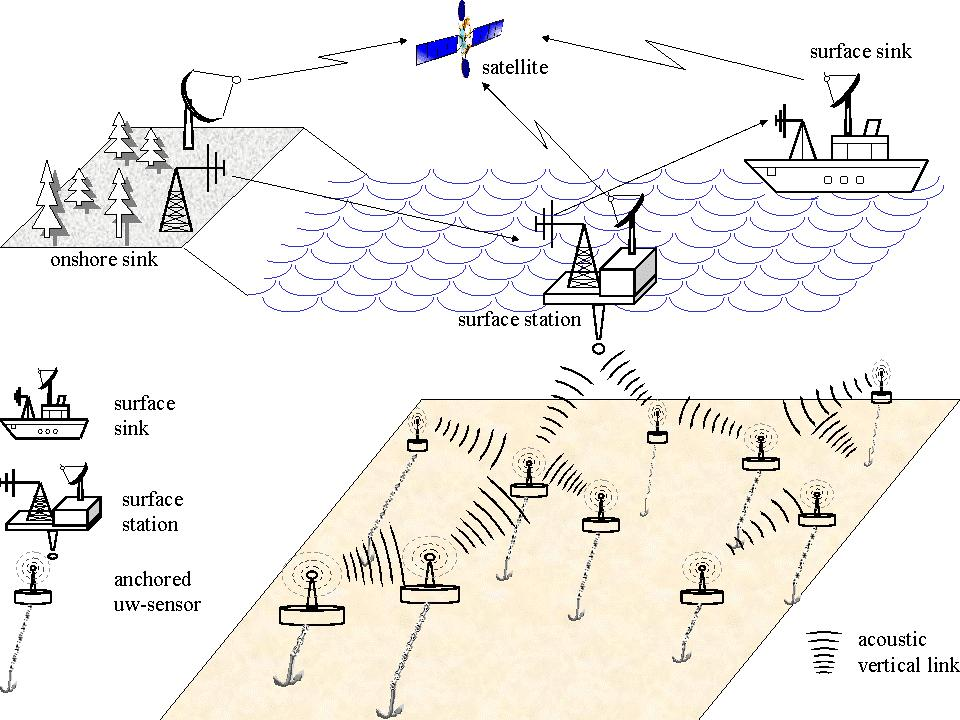
\includegraphics[scale=0.3]{3D_arch.jpg}
	\caption{ Topologia nodi fissi 3D}
	\label{fig:}
\end{figure}

In questo caso i sensori debbono svolgere una funzione che richiede loro di disporsi a diverse profondita'. Per effettuare il posizionamento, e' possibile agganciare i sensori a delle boe galleggianti (che pero' risultano visibili in superficie e possono essere d'intralcio alla navigazione) oppure e' possibile agganciare direttamente il sensore ad una boa ed ancorare la stessa, tramite una corda, al fondo marino.  In questo modo e' possibile regolare dinamicamente la profondita' del sensore tramite motore elettrico in grado di allungare/accorciare la corda d'ancoraggio. Come evidente dall'immagine, in questa topologia manca del tutto il concetto di uw-sink. I sensori sono costretti a comunicare con la stazione di superficie in modalita' multi-hop e quindi debbono necessariamente implementare le funzionalita' tipiche di un router, con l'onere computazionale aggiuntivo che cio'comporta. A causa delle correnti marine, spesso i nodi di questa tipologia di reti subiscono modifiche non volute al proprio posizionamento. Diventa quindi fondamentale la comunicazione e la collaborazione fra i sensori di questa rete in modo che ciascuno di essi possa riconfigurare in corso d'opera la propria profondita', in funzione di due obbiettivi primari:
\begin{itemize}

 \item Mantenere la copertura totale nel rilevamento della colonna interessata dalla raccolta dati dei sensori

\item Mantenere la connessione della topologia di rete, ovvero far si che esista, per ciascun nodo, un percorso fruibile verso la stazione di superficie
\end{itemize}

La terza e ultima topologia di rete presa in considerazione espande le caratteristiche delle prime due configurazione analizzate introducendo la presenza di nodi mobili all'interno della rete (Autonomous Underwater Vehicle, AUV).

\begin{figure}[h]
	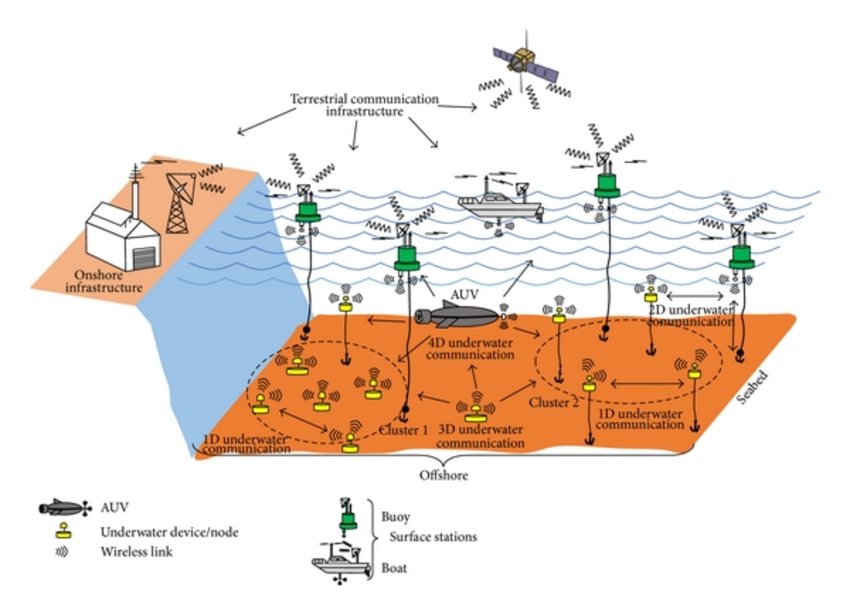
\includegraphics[width=\linewidth]{auv_arch.png}
	\caption{ Topologia comprendente nodi mobili}
	\label{fig:}
\end{figure}

L'introduzione di nodi mobili all'interno della rete espande enormemente le capacita' di una UWSN, dato anche il costo relativamente basso di un AUV equipaggiato con diversi sensori. La presenza di nodi mobili nella rete permette, ad esempio, l'adaptive sampling, ovvero la possibilita' di posizionare adattativamente i sensori mobili presso un particolare punto d'interesse, variando la densita' di sensori presenti in quella data zona. Inoltre, facendo riferimento alle questioni sorte nella trattazione della rete tridimensionale di nodi fissi, appare chiaro come un AUV possa, data la sua maggior liberta' di movimento, ovviare facilmente a deficit nella copertura di un area o ad eventuali buchi che si vengono a creare nella rete (ad esempio andando a sostituire un nodo fisso malfunzionante andando a posizionarsi in prossimita' di questo).
Esistono in commercio diversi tipi di AUV, fra i quali ricordiamo:
\begin{itemize}

\item i drifters, ovvero veicoli che viaggiano seguendo la corrente oceanica in cui sono immersi, con la possibilita' di variare solamente la propria
profondita d'azione

\item i gliders (``alianti''), dotati di timone di coda e di ali laterali, i quali possono variare la propria linea di galleggiamento in modo da alimentare la propria spinta propulsiva in avanzamento

\item AUV simili a veri e propri sottomarini in miniatura, dotati di propulsione elettrica tramite eliche

\end{itemize}
\begin{figure}[H]
    \centering
	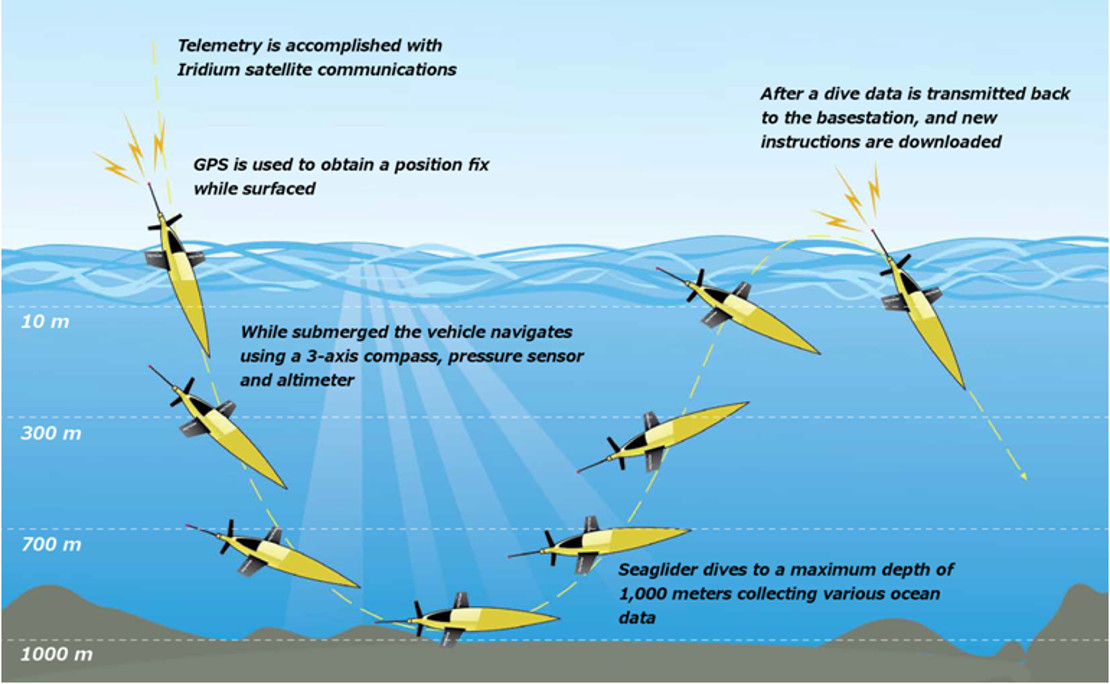
\includegraphics[width=\linewidth]{glider.jpg}
	\caption{ Esempio di funzioamento di un glider}
	\label{fig:}
\end{figure}


\begin{figure}[H]
    \centering
	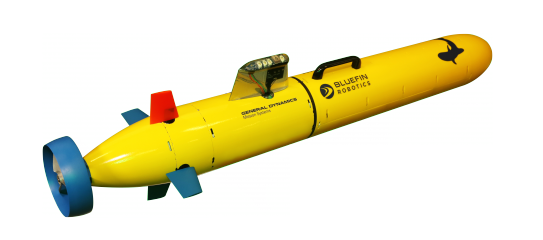
\includegraphics[width=\linewidth]{auv.png}
	\caption{ Esempio di AUV}
	\label{fig:}
\end{figure}

\subsection{SUNSET: Sapienza Underwater }

SUNSET, acronimo di Sapienza Underwater Networking framework for underwater Simulation and Emulation and real-life Testing, e' un framework per lo sviluppo ed il testing di protocolli per reti underwater ed e' stato scelto come ambiente di sviluppo e valutazione del protocollo di localizzazione ivi analizzato \cite{sunset}.\newline
SUNSET e' basato sul simulatore di reti open-source ns-2 e su una sua estensione, ns2-Miracle, ampiamente utilizzati in quest'ambito scientifico, il che permette agli sviluppatori gia' usi a questi strumenti una rapida transizione verso l'utilizzo di questo framework.
SUNSET prevede tre modalita' di utilizzo: simulation, emulation e real-life testing.
La prima permette di simulare preventivamente il funzionamento della rete, in maniera totalmente indipendente dall'hardware che verra' utilizzato nel test reale, fornendo agli sviluppatori la possibilita' di testare le proprie soluzioni protocollari in un ambiente controllato variando una moltitudine di parametri ambientali e di configurazioni. Fra queste, ricordiamo le diverse soluzioni per quanto concerne il modello di trasmissione dei segnali acustici in acqua: formule empiriche ( come il modello di Urick), il simulatore di propagazione Bellhop (incluso tramite WOSS) e dati reali del canale replicabili all'interno del simulatore.
\newline
Una delle caratteristiche peculiari che rendono SUNSET una soluzione d'avanguardia nel settore consiste nel rendere praticamente immediato il passaggio dall'ambiente simulativo a quello emulativo/real-life. Difatti, al costo di lievi modifiche al codice sorgente, i protocolli sviluppati possono essere impiegati indipendentemente sia nella modalita' di simulazione che nelle altre due modalita'. Questa caratteristica garantisce a SUNSET un enorme vantaggio rispetto ad altre soluzioni software operanti nello stesso ambito. Basti pensare al costo, in termini di tempo e denaro, del testing reale di una nuova tecnologia in ambito di UWSNs, comprendente come voce non trascurabile la traduzione delle tecnologie sperimentate nell'ambiente simulativo in strumenti operativi concretamente fruibili. SUNSET rende praticamente trascurabile lo sforzo da parte degli sviluppatori per questa operazione.
\newline
Nello sviluppo di SUNSET si e' voluta separare la componente riguardante l'implementazione della pila protocollare dai moduli utili al controllo della componentistica reale in modalita' di emulazione. Pertanto, lo sviluppatore puo' modificare, ad esempio, la logica di funzionamento di un protocollo senza intaccare in alcun modo i driver di controllo dei vari device e viceversa.
Una novita' introdotta nell'ultima versione di SUNSET, identificata' dal termine "backseat-driver", ha come scopo dare maniera agli sviluppatori di modificare, in real-time durante lo svolgimento di un test sul campo, la configurazione di una rete di sensori underwater gestita tramite SUNSET. Si puo', ad esempio, modificare la topologia di rete, spegnendo od accendendo dei nodi, oppure mutare i parametri di funzionamento di un protocollo.
\newline
SUNSET supporta in maniera ottimale ben 5 modem acustici in circolazione, oltre a numerosi sensori disponibili in commercio, offrendo una piattaforma unitaria sia per il controllo delle funzionalita' di rete sia per il data sensing. Non ultima l'efficienza in termini di costo computazionale, che permette a SUNSET si essere eseguito su piattaforme dotate di risorse di calcolo limitate (ad esempio Gumstix ed altri sistemi ARM-based).

\subsection{Prospettiva sul ruolo dei dispositivi mobili nelle UWSNs}
I veicoli sottomarini, di cui sopra abbiamo dato una rapida panoramica, stanno rivoluzionando l'approccio allo studio ed al monitoraggio dell'ambiente marino. \newline Sebbene questi veicoli necessitino di essere sganciati in acqua solitamente da una nave, una volta disposti nell'ambiente marino possono lavorare in maniera autonoma, non avendo necessita' di essere costantemente controllati dall'uomo durante le loro operazioni. \newline Questo ha permesso nel recente passato la realizzazione di missioni volte all'acquisizione di dati scientifici in zone altrimenti inaccessibili alla navigazione ( come ad esempio il deployment di AUVs sotto la lastra di ghiaccio artica \cite{wadhams}), migliorando inoltre la risoluzione spaziale e temporale rispetto a misurazioni effettuate in maniera indiretta.\newline
In questo paragrafo ci concentreremo sulla descrizione degli AUVs.
Come anticipato nel paragrafo percendente, gli AUVs sono veicoli sottomarini che non necessitano di equipaggio umano. Posseggono un proprio sistema di propulsione, vengono solitamente sganciati da una nave e possono operare indipendentemente da questa, per un periodo che va dalle ore all'ordine dei giorni. Molti degli AUVs sviluppati hanno la forma di siluro, sebbene ne esistano anche di forme diverse (adatti a particolari tipi di fondali e movimento).\newline
Il vantaggio principale degli AUVs rispetto ai gliders e' la possibilita' di navigare seguendo una traiettoria lineare, rendendoli adatti a missioni che richiedono il mantenimento di un'altezza costante.
Difatti, l'utilizzo piu' rilevante di questi veicoli  avviene in studi che riguardano la zona di interfacciamento del fondale marino con la colonna d'acqua soprastante o direttamente lo studio del fondale.  In questa zona dell'ambiente sottomarino si concentrano gli organismi bentonici e avvengono i processi di sedimentazione di materiali sul fondale. 
Gli AUVs, grazie al loro particolare movimento, possono quindi effettuare il monitoraggio di questa zona mantenendosi ad una profondita' costante, potendo navigare anche molto vicini al fondale ($\leq$ 5m). \newline
In generale, la possibilita' di navigare in linea retta ad una distanza ravvicinata dal fondale marino permette, utilizzando strumenti quali sonar a scansione laterale (Side Scan Sonar, SSS), ecoscandagli multifascio (Multi-Beam Echosounders, MBES) e profilatori sismici di sedimenti (Sub Bottom Profilers, SBP) e' possibile mappare e generare immagini del profilo del fondale marino in maniera molto piu' precisa rispetto ai dati ottenuti utlizzando strumenti posti su navi ( fino a due ordini di grandezza piu' precisi). \newline 
Non va tralasciato l'aspetto economico che sta rendendo sempre piu' appetibile l'uso di AUVs nelle missioni in ambito marino. L'elevato costo legato al noleggio/acquisto di imbarcazioni per svolgere queste missioni spinge ricercatori e aziende ad cercare di sostituirle con meno costosi AUVs. Inoltre, la natura "autonoma" degli AUVs li rende perferibili anche rispetto ai ROVs (Remotely Operated Vehicles), dispositivi sottomarini controllati in real-time da un operatore umano (e che quindi richiedono la presenza della nave d'appoggio nelle immediate vicinanze del veicolo). Non e' difficile immaginare uno scenario operativo in cui un AUV opera in autonomia in una data area e nel contempo la nave d'appoggio svolge un'operazione del tutto differente, permettendo, rispetto ai ROVs, un significativo aumento dei dati raccoglibili nello stesso tempo di utilizzo della nave d'appoggio. \newline
Dato che il pregio fondamentale degli AUVs consiste nella loro capacita' di muoversi in autonomia, molto del lavoro di sviluppo di questi sistemi riguarda la progettazione di un sistema di navigazione preciso ed affidabile. In un sistema del genere, la localizzazione e' una componente fondamentale, oltre che essere argomento di questo elaborato.
Gli AUVs, nel loro spostamento, seguono solitamente un percorso prestabilito e sono capaci di navigare utilizzando diverse soluzioni tecniche, che vengono di seguito discusse.


\section{Sistemi di localizzazione acustica sottomarini}
Appare chiaro come, sia per sensori fissi che per AUVs, i dati da essi raccolti abbiano molto spesso valore solamente se integrati dall'informazione circa la posizione esatta nella quale gli stessi sono stati rilevati. Inoltre alcuni servizi, quali ad esempio la copertura di zone d'ombra che dinamicamente si vengono a creare in una rete, non sarebbero possibili senza una precisa localizzazione degli elementi stessi della rete.
Vediamo in breve le principali tecniche di localizzazione esistenti.

\subsection{Tecniche di localizzazione}
Per localizzazione intendiamo quella procedura atta a determinare la posizione di un sensore, fisso o mobile, in termini di coordinate spaziali. Le coordinate possono riferirsi ad un sistema di riferimento globale (es. latitudine, longitudine e profondita') oppure relative ad un sistema di coordinate locali (come ad esempio coordinate relative ad un particolare sensore preso come origine di un sistema di riferimento cartesiano).
\par
Per qualunque sistema di localizzazione, due paramentri sono fondamentali per valutarne l'affidabilita':
\begin{itemize}
    \item Accuratezza: quanto la posizione calcolata sia distante dalla posizione reale
    \item Precisione: quanto le misurazioni effettuate siano fra loro consistenti
\end{itemize}
Ad esempio, un sistema di localizzazione con accuratezza 3$m$  e precisione dell'80\% delle misurazioni ci rassicura sul fatto che 8 volte su 10 la posizione che esso calcolera' sara' errata di al piu' 10$m$.
\par
Nei sistemi di localizzazione, le misure principali richieste per effettuare i calcoli necessari sono delle distanze relative. Queste sono calcolabili utilizzando il ToA, Time-of-Arrival, ovvero il tempo di propagazione richiesto ad un segnale per compiere il tragitto da un emettitore ad un ricevente. Conoscendo la velocita' di propagazione del segnale nel mezzo specifico, possiamo calcolare la distanza fra sorgente e destinatario del segnale.
Possiamo categorizzare i sistemi di localizzazione in alcune classi principali \cite{trilateration}:
\begin{itemize}
    \item One-way ToA: la distanza viene calcolata utilizzando la propagazione di un solo segnale (e richiedono percio' elevata sincronizzazione temporale tra i due nodi):
    \[dist_{ij}\ =\ (t_2-t_1)*v\]
    \item Two-way ToA: la distanza viene calcolata misurando il RTT di un segnale e non richiede sincronizzazione tra i nodi:
    \[dist_{ij}\ =\ \frac{(t_4-t_1)-(t_3-t_2)}{2}*v\]
    \item Time Difference of Arrival (TDoA): due segnali con differenti velocita', il primo di velocita' $v_1$ inviato all'istante $t_1$ e ricevuto a $t_2$ e l'altro di velocita' $v_2$ inviato a $t_3 = t_1 + t_{wait}$ e ricevuto a $t_4$. Non si richiede sincronizzazione tra i due nodi, ma c'e' la necessita' di due sorgenti differenti di segnale.
    \[dist = (v_1 - v_2)*(t_4 - t_2 - t_wait)\]
    \item Angle of Arrival (AoA): sistema che richiede un array di antenne o microfoni. La ricezione dello stesso segnale da ciascun ricevitore con caratteristiche differenti (tempo d'arrivo, fase, ampiezza) consente di calcolare l'angolo fra il segnale ed un certo punto di riferimento, oltre alla distanza.
    \item Received Signal Strength (RSS): sistemi in cui il calcolo della distanza dall'emettitore del segnale avviene conoscendo la potenza iniziale del segnale, quella con cui lo si e' ricevuto e il modello che descrive il decadimento del segnale con la propagazione.
\end{itemize}
Il sistema USBL, di cui parleremo subito dopo, appartiene alla categoria di sistemi di localizzazione AoA, mentre quelli SBL e LBL sono di tipo Two-way ToA o Onw-way ToA.
Questi ultime due classi di sistemi fanno ricorso, per il calcolo effettivo della posizione, al metodo matematico della trilaterazione.
Conoscendo la distanza dell'oggetto da localizzare rispetto ad un nodo fisso, l'oggetto deve necessariamente giacere sulla superficie di una sfera (in due dimensioni, sul perimetro di una circonferenza) centrata nel nodo fisso ed avente raggio pari alla distanza calcolata. Possiamo quindi impostare un sistema di tante equazioni di secondo grado (equazione della superficie di una sfera) quanti sono i nodi fissi da cui conosciamo la distanza. Risolvendo il sistema (con tecniche di cui parleremo nella parte dedicata al protocollo sviluppato) si puo' ottenere la posizione dell'oggetto d'interesse.

\subsection{LBL, USBL, SBL}
I sistemi acustici di localizzazione sottomarina possono essere classificati in tre categorie, in base al principio di funzionamento utilizzato ed alla modalita' con cui viene approntato il sistema. \cite{underwaterpositioning} \newline
In primis, consideriamo i sistemi LBL (Long-baseline).  Il loro funzionamento dipende dal posizionamento di 3 o piu' transponders vengano piazzati sul fondale marino (o ad una certa altezza dal fondale), la cui posizione deve essere nota in maniera precisa. 
I transponders vengono posti solitamente al margine dell'area operativa dei veicoli che si intende localizzare, ad una distanza abbastanza elevata ciascuno dall'altro. Sul nodo mobile viene montato un segnalatore che invia un segnale acustico ai transponders. Questi ultimi ricevono il segnale e lo reinviano al veicolo. Tramite il time-of-flight del segnale, il veicolo conosce la propria distanza da ciascuno dei transponders e puo' effettuare la localizzazione (ad esempio tramite triangolazione o trilaterazione).

\begin{figure}[H]
    \centering
	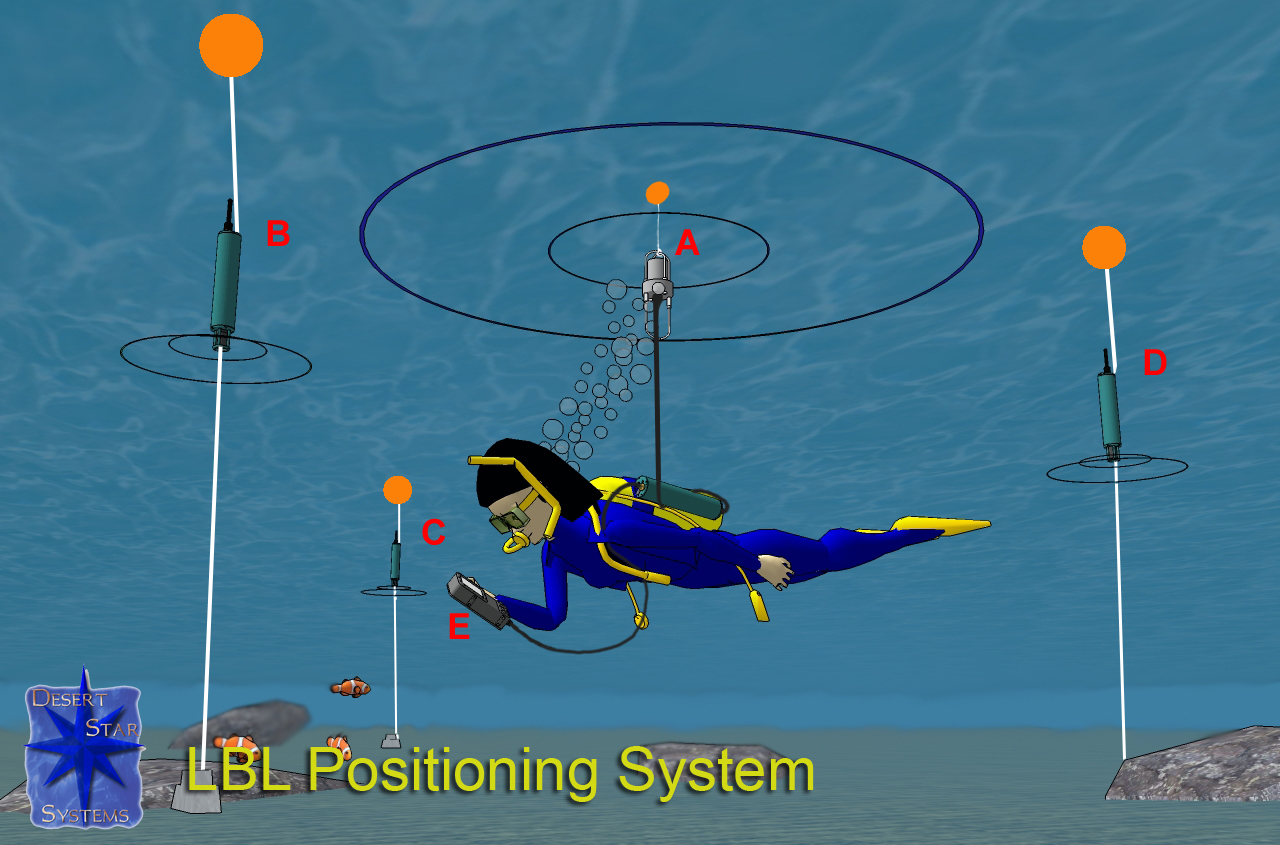
\includegraphics[scale=0.25]{LBL.jpg}
	\caption{ Esempio di localizzazione LBL}
	\label{fig:LBL}
\end{figure}
\newpage

I sistemi USBL (Ultra Short Base-line ) sfruttano invece un'array di trasduttori, montati solitamente sul fondo di una barca. L'AUV invia un segnale che viene ricevuto da questi trasduttori i quali, dal time-of-flight, calcolano la distanza del nodo mobile dall'imbarcazione e, utilizzando la differenza di fase fra il segnale ricevuto dai diversi trasduttori, ne calcolano anche la direzione. Dalla combinazione di distanza e direzione si ottiene la posizione dell'AUV, che pero' risulta notevolmente meno precisa di quella ottenuta con metodo LBL ( ma richiede un segnale in meno). L'errore nel posizionamento dipende fondamentalmente dalle imprecisioni nella direzione calcolata (in particolare quando l'AUV e' lontano dai trasduttori).\newline
In ultimo , i sistemi SBL (Short Base-line), simile a quelli USBL per la mancanza di transponders fissati al fondale ma che sfruttano un meccanismo simile a quello degli LBL. Infatti, in questi sistemi, 3 o piu' transponders vengono collegati ad un sistema di controllo centrale ed immersi in acqua, solitamente attaccati sul fondo di una barca o di un molo. Uno di questi transponders invia un segnale che viene ricevuto dal nodo mobile, che a sua volta risponde inviando un segnale a tutti i transponders. Dai tempi di propagazione viene ricavata la distanza dell'AUV , utilizzata poi nel calcolo della localizzazione come nel caso dei sistemi LBL.

\begin{figure}[H]
	\centering
	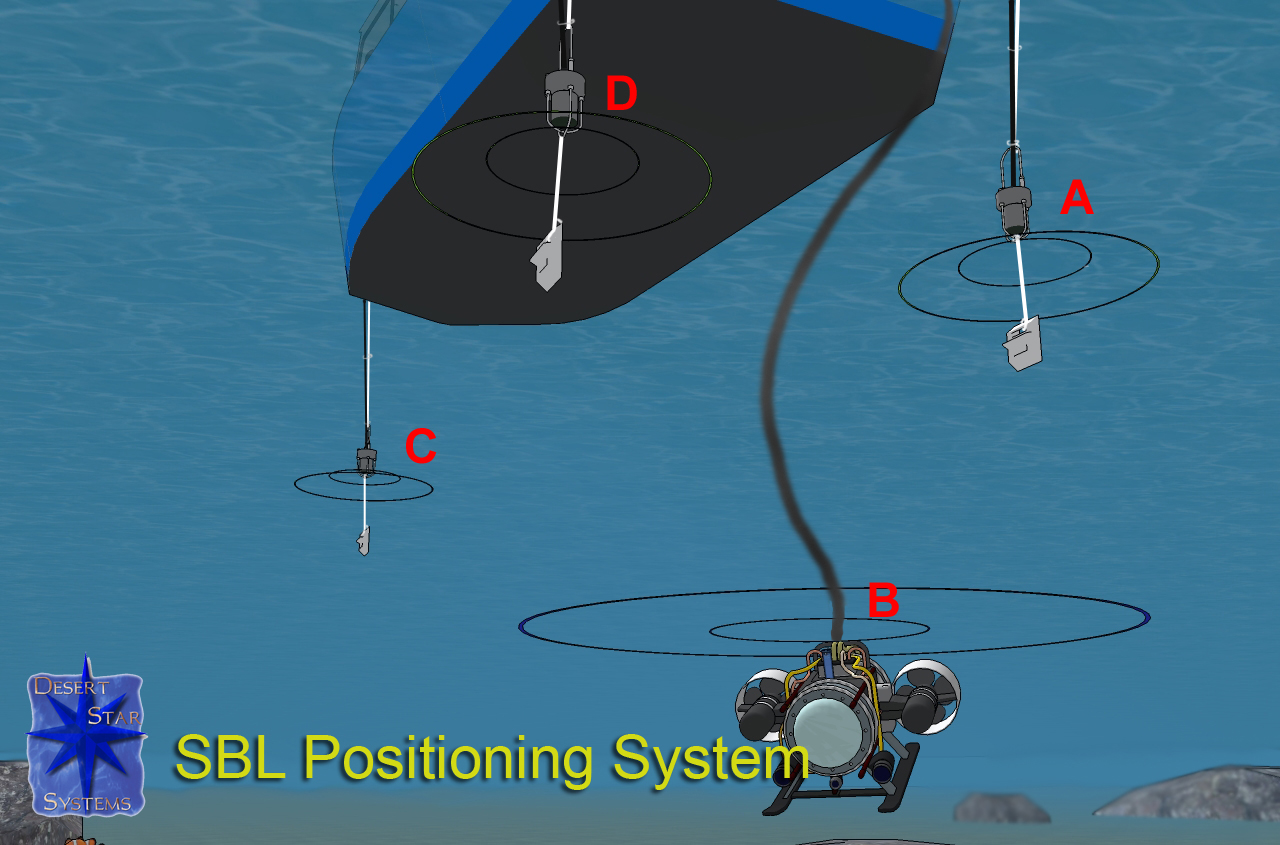
\includegraphics[scale=0.25]{SBL.jpg}
	\caption{ Esempio di localizzazione SBL}
	\label{fig:SBL}
\end{figure}


\par
In quest'elaborato si e' scelto di replicare un sistema di localizzazione sul modello di quelli LBL. Nel nostro caso, al posto dei transponders, vengono utilizzati dei nodi fissi (intesi come sensori fissati o agganciati al suolo) e non vengono scambiati dei semplici e brevi segnali acustici ma dei veri e propri pacchetti di rete. In questo modo, la localizzazione di un nodo mobile avviene contemporaneamente allo scambio di informazioni di altro tipo (ad esempio comandi di riconfigurazione inviati dall'AUV ai nodi fissi o dati raccolti dai nodi fissi all'AUV), al costo della sola aggiunta di un nuovo header ai pacchetti trasmessi.  

\section{Contributo dell'elaborato di tesi}
Il lavoro esposto in questo elaborato ha avuto una duplice finalita'.
In primis, si e' cercato di creare un modello di movimento, che fosse il piu' possibile attendibile, per un AUV realmente esistente e disponibile in commercio, MARTA (acronimo di MArine Robotic Tool for Archaeology). In questo modo le simulazioni successivamente effettuate hanno sicuramente goduto di un maggior grado di aderenza ad un possibile scenario reale di applicazione.
\par
Il secondo contributo dell'elaborato di tesi e' un sistema di localizzazione per un AUV.
Il sistema di localizzazione e' stato appunto pensato come protocollo da inserire nella pila protocollare di un nodo mobile di una rete, sfruttando l'architettura del network gia' esistente in una UWSN per effettuare il calcolo della posizione di un veicolo (evitando quindi di introdurre un'infrastruttura ad hoc).
Il protcollo sviluppato si basa sui sistemi di localizzazione LBL, di cui gia' e' stato spiegato a grandi linee il comportamento. La fattibilita' di un sistema del genere e' garantita dall'esistenza in commercio di modem acustici che garantiscono la possibilita' di inviare pacchetti con header personalizzato e sono molto precisi nella misurazione delle tempistiche di invio e ricezione dei pacchetti stessi. Nondimeno, sono gia' in produzione da anni sistemi LBL di notevole precisione \cite{lblsonardyne} che comprovano la concreta realizzabilita' del sistema quivi sviluppato.